\documentclass{beamer}

\usepackage{biblatex}
\setbeamerfont{footnote}{size=\tiny}

\input{header-presentation}
\title[FPGA for BING!]{A Reconfigurable Fabric for Accelerating Large-Scale Datacenter Services}
\author[bobzhou@bu.edu]{Reviewed by Boyou Zhou}
\date[\today]{\today}

\begin{document}
\maketitle

\section*{FPGA for BING!}

\begin{frame}{Comparison Between GPP, FPGA, and ASIC}
    \begin{figure}
        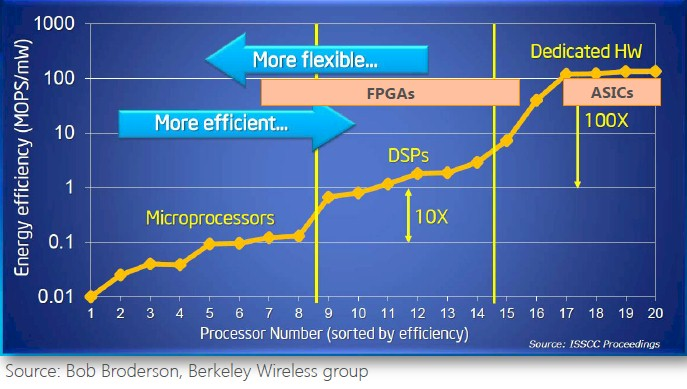
\includegraphics[width=4in]{img/microsoft-fpga-vs-cpu-vs-asic.png}
        \caption{FPGA, FPGA, and ASIC comparison from Microsoft\footcite{http://www.theplatform.net/2015/03/30/why-intel-might-buy-fpga-maker-altera}}
        \label{fig:comparison}
    \end{figure}
\end{frame}

\begin{frame}{Blocks Everywhere}
  \begin{block}{Blocks are better?}
    \begin{itemize}
    \item Everything in beamer seems to look better in blocks
    \item So, the default slide has a block and an itemized list
      \begin{itemize}
      \item You can also nest itemized lists
      \end{itemize}
    \end{itemize}
  \end{block}
\end{frame}

\begin{frame}{Column Slide}
  \begin{columns}[b]
    \column{0.60\textwidth}
    \begin{block}{First \textbf{BIG} Column}
      \begin{itemize}
      \item You can split content into columns
      \item Column size is governed manually
      \item Column alignment (here \texttt{b}, bottom) can also be specified
      \end{itemize}
    \end{block}

    \column{0.35\textwidth}
    \begin{block}{Second {\tiny little} Column}
      \begin{itemize}
      \item ALPHA
      \item BRAVO
      \item CHARLIE
      \item DELTA
      \item ECHO
      \end{itemize}
    \end{block}
  \end{columns}
\end{frame}
\end{document}
